\section{System Architecture}

\begin{figure}[h!]
	\centering
    	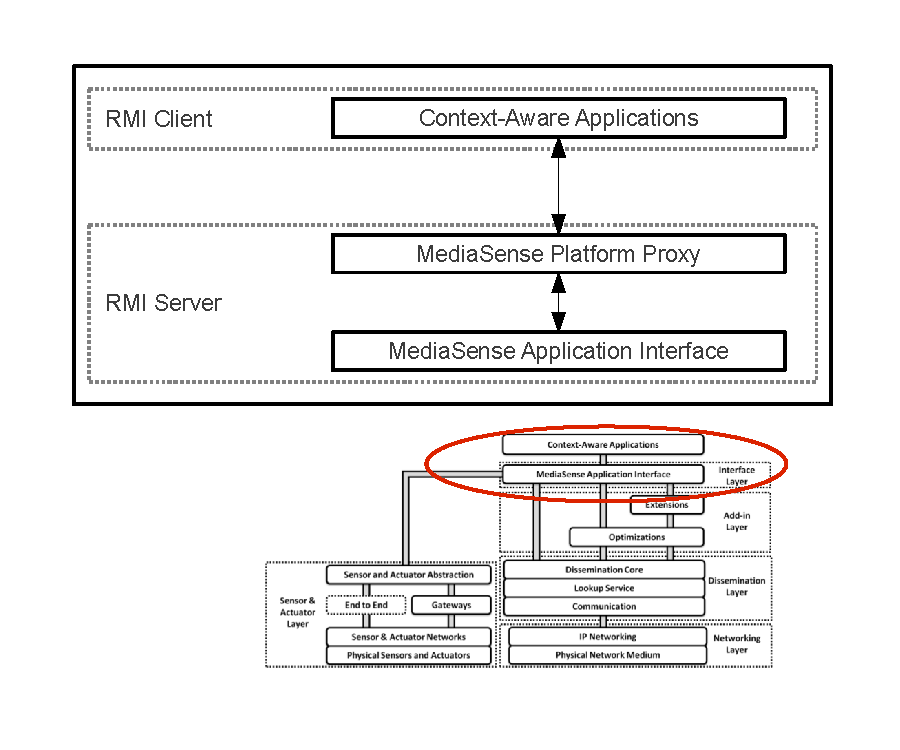
\includegraphics{part_6/artefact_description/changes.pdf}
		\caption{Figure showing how MediaSense Platfrom Proxy and application communicate with each other and where the RMI client and server is located in the architecture.} 
		\label{ds}
\end{figure}

\subsection{Network Overlay}
The network overlay handles the communication with other nodes and stores peer data in a database. The overlay has remained the same as in the old version of MediaSense and thus satisfies the requirement that the overlay should remain unmodified.

\subsection{MediaSense Messages}
MediaSense communicates with other nodes in the network by sending and receiving messages. Messages have a scope and can either be sent to a specific application or to all applications at a peer node. 
To create an application scoped message the application ID is sent as an argument to the constructor and the messages are then sent to the application that is identified with this ID. 
Messages can also be sent as peer messages, the message is sent to all applications on the receiving peer-node. In the original version of MediaSense, because every instance of the platform only ran one application, the messages had no scope and thus the applications would receive all messages. 
In the version that has been developed in this project, the dissemination core can redirect messages to specific applications. With the possibility to send messages to specific applications, the new version of MediaSense fulfills the requirement that applications should have scope.

\subsection{Dissemination Core}
The Dissemination layer in MediaSense includes different components, dissemination core and lookup service. The lookup service finds and resolves other entities who connects to the network. The dissemination core works as a router for the messages. When the platform is receiving messages the dissemination core handles these messages and sends them to the applications that are interested in those messages. If an application ID is specified, the message will be sent to the application with this ID. If the message type is set to be a peer message, the message will be sent to all applications connected to the platform instead. The dissemination core and the use of RMI satisfies the requirement that the artefact should handle several applications.

\subsection{MediaSense Platform Interface Layer}
The MediaSense Platform Interface Layer initiates the core components of the MediaSense platform, the Dissemination Core, the Pgrid lookupservice, and Pgrid's module for network communication. In the old version, it was also used to expose the functionality of the MediaSense Platform to the applications. In the new version, this component is only used by the RMI server. The client applications now access this functionality through the RMI Proxy which in turn calls the Interface Layer. This satisfies the requirement that applications should have an interface to the platform and that they should use a common network overlay.

\subsection{MediaSense Platform RMI Proxy}
This component is a RMI server that register itself to the RMI registry and makes it possible for RMI client to connect to it. The RMI proxy provides methods so the applications can communicate with the RMI server which is calling methods in the provided MediaSense Platform Interface Layer. The RMI server is acting as a shaded API so applications can call methods that are provided by MediaSense. This component makes it possible for several applications to connect to it and, therefore, only one MediaSense instance is needed for communication with the platform. This allows MediaSense to be run as a background process and thus satisfies the requirement that MediaSense should be able to run as a daemon.

\subsection{MediaSense Application Interface}
The application interface is used when a developer is developing an application. The developer extends this interface to get access to functionality that is needed for applications running on MediaSense. 
To create a MediaSense application, a few things are required. 

\begin{itemize}
  \item An application extending the interface must define its own unique application ID. This ID can be used to set the scope of a message to a specific application. 
  \item Applications must register what types of messages they are interested in receiving using the RMI Proxy's registerListener method. 
  \item An application needs to register itself on the platform by sending a reference of itself to be stored in the platforms list of applications. This is done by providing the applications ID as a parameter to the method called registerApplication in MediaSense Platform RMI proxy.
  \item The application interface contains one method that developers need to override, called handleMessage. This method is used for handling incoming messages to the application and responsible for responding to these messages. 
\end{itemize}

To communicate with the MediaSense platform, an application must first know the IP address of the device where the RMI registry is located. If the platform runs on the same device as the applications, an arbitrary port is used. After connecting to the registry, the RMI Proxy is located through a lookup on the registered name \emph{mediasense} and an instance of it is saved in the application. When the application interface needs to communicate with the platform a method called getPlatformInterface is available which returns the instance of the RMI Proxy, on which all calls to the platform then can be done.

